% Part: sets-functions-relations
% Chapter: relations
% Section: graphs

\documentclass[../../../include/open-logic-section]{subfiles}

\begin{document}

\olfileid[pt]{sfr}{rel}{grp}
\olsection{Grafos}

Um \emph{grafo} é um diagrama no qual pontos---chamados ``nós'' ou
``vértices'' (plural de ``vértice'')---são conectados por arestas. Grafos
são uma ferramenta onipresente em matemática discreta e em ciência da computação.
São incrivelmente úteis para representar e visualizar
relações e estruturas, desde coisas concretas como redes de
vários tipos até estruturas abstratas como os possíveis resultados de
decisões. Existem muitos tipos diferentes de grafos na literatura
que diferem, p.ex., quanto a se as arestas são direcionadas ou
não, têm rótulos ou não, se pode haver arestas de um nó para o
mesmo nó, múltiplas arestas entre os mesmos nós, etc. \emph{Grafos
  direcionados} têm uma conexão especial com relações.

\begin{defn}[Grafo direcionado]
Um \emph{grafo direcionado} $G = \tuple{V, E}$ é um conjunto de
\emph{vértices}~$V$ e um conjunto de \emph{arestas}~$E \subseteq V^2$.
\end{defn}

\begin{explain}
De acordo com nossa definição, um grafo é simplesmente um conjunto junto com uma
relação nesse conjunto. Claro, ao falar de grafos, é natural
esperar que sejam representados graficamente: podemos desenhar um
grafo conectando dois vértices~$v_1$ e $v_2$ por uma seta sse
$\tuple{v_1, v_2} \in E$. A única diferença entre uma relação por
si só e um grafo é que um grafo especifica o conjunto de vértices,
isto é, um grafo pode ter vértices isolados. O ponto importante,
porém, é que toda relação~$R$ em um conjunto~$X$ pode ser vista como um
grafo direcionado $\tuple{X, R}$, e reciprocamente, um grafo
direcionado~$\tuple{V, E}$ pode ser visto como uma relação $E \subseteq V^2$ com
o conjunto $V$ explicitamente especificado.
\end{explain}

\begin{ex}
O grafo $\tuple{V, E}$ com $V = \{1, 2, 3, 4\}$ e $E =
\{\tuple{1,1}, \allowbreak \tuple{1, 2}, \allowbreak \tuple{1, 3},
\allowbreak \tuple{2, 3}\}$ se parece com isto:
\begin{align*}
& 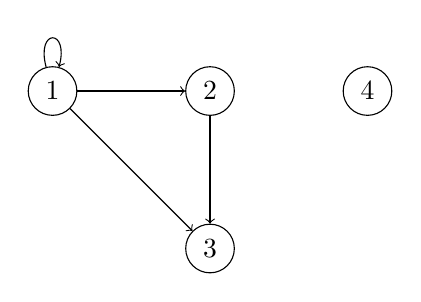
\begin{tikzpicture}[->,node distance=2cm]
  \node[draw,circle] (A) {$1$};
  \node[draw,circle] (B) [right of=A] {$2$};
  \node[draw,circle] (C) [below of=B] {$3$};
  \node[draw,circle] (D) [right of=B] {$4$};
  \draw (A) to [loop above]  (A);
  \draw (A) to  (B);
  \draw (A) to  (C);
  \draw (B) to  (C);
  \end{tikzpicture}
\intertext{Este é um grafo diferente de $\tuple{V', E}$ com $V' =
  \{1, 2, 3\}$, que se parece com isto:}
& 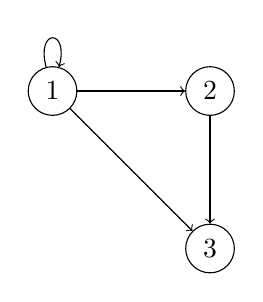
\begin{tikzpicture}[->,node distance=2cm]
  \node[draw,circle] (A) {$1$};
  \node[draw,circle] (B) [right of=A] {$2$};
  \node[draw,circle] (C) [below of=B] {$3$};
  \draw (A) to [loop above]  (A);
  \draw (A) to  (B);
  \draw (A) to  (C);
  \draw (B) to  (C);
  \end{tikzpicture}
\end{align*}
\end{ex}

\begin{prob}
  Considere a relação menor ou igual a~$\le$ no conjunto $\{1,
  2, 3, 4\}$ como um grafo e desenhe o diagrama correspondente.
\end{prob}

\end{document}
